\section{Muh. Rifky Prananda(1174017)}
\subsection{Instalasi Map Server}
\begin{enumerate}
    \item Download terlebih dahulu map servernya. Untuk webnya bisa \href{https://mapserver.org/}{Klik disini} atau \href{https://ms4w.com/}{Klik disini} Untuk windows.
    \hfill\break
    \begin{figure}[H]
		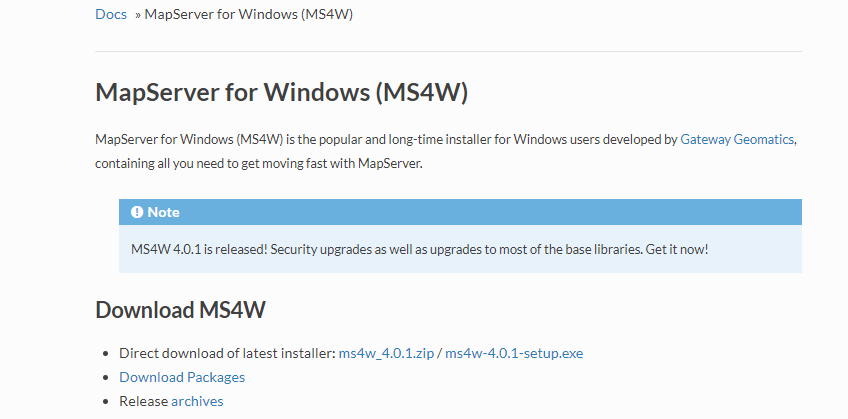
\includegraphics[width=4cm]{figures/1174017/4/Capture.png}
		\centering
		\caption{Halaman map server untuk windows}
    \end{figure}
    \item Setelah di download, bisa langsung melakukan Instalasi. Untuk versi windows bisa saya sarankan mendownload yang .exe agar lebih mudah saat instalasi.
    \hfill\break
    \begin{figure}[H]
		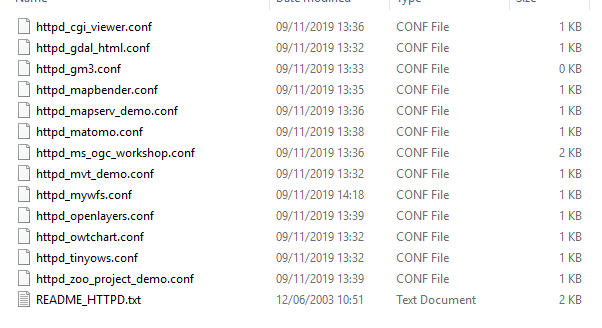
\includegraphics[width=4cm]{figures/1174017/4/Capture2.png}
		\centering
		\caption{File yang telah didownload}
    \end{figure}
    \item Instal vcredist 2017, untuk bisa menjalankan map server. untuk linknya bisa \href{https://support.microsoft.com/id-id/help/2977003/the-latest-supported-visual-c-downloads}{Klik disini}
\end{enumerate}
\subsection{Konfigurasi Map Server}
Jika telah selesai melakukan instalasi kita akan melakukan konfigurasi
\begin{enumerate}
  \item Buka folder ms4w tadi
  \hfill\break
    \begin{figure}[H]
		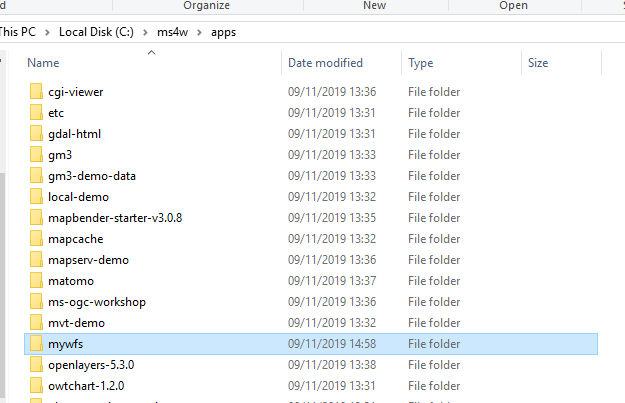
\includegraphics[width=4cm]{figures/1174017/4/1.png}
		\centering
		\caption{Localdisk C}
    \end{figure}
    \hfill\break
    \begin{figure}[H]
		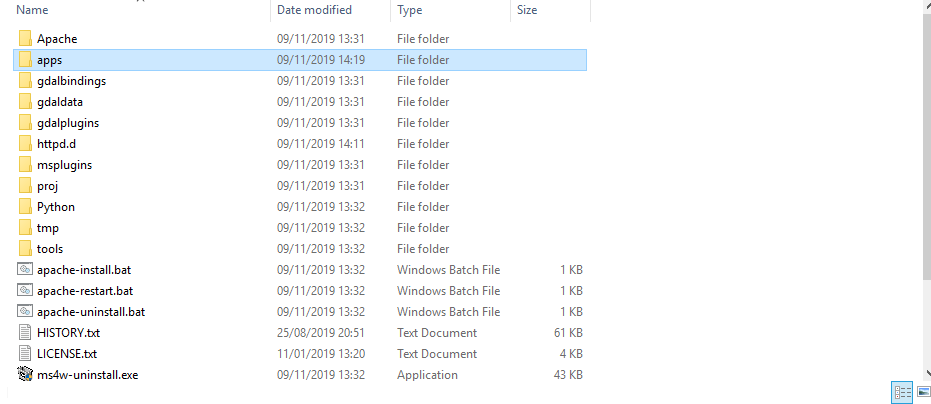
\includegraphics[width=4cm]{figures/1174017/4/2.png}
		\centering
		\caption{Isi Folder ms4w}
    \end{figure}
  \item Masuk ke folde apache
  \hfill\break
    \begin{figure}[H]
		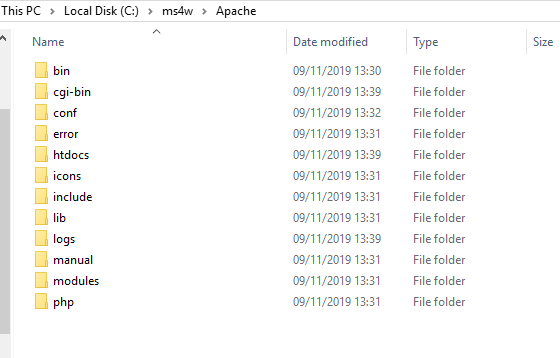
\includegraphics[width=4cm]{figures/1174017/4/3.png}
		\centering
		\caption{Isi Folder Apache}
    \end{figure}
  \item Masuk ke folder conf
  \hfill\break
    \begin{figure}[H]
		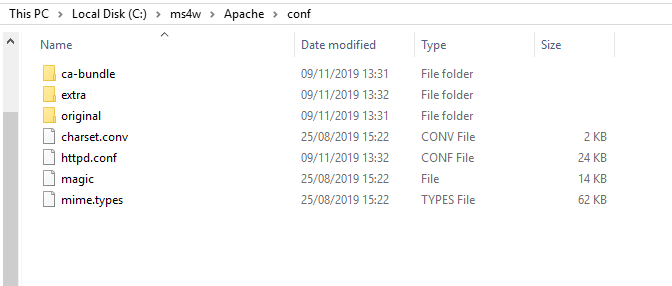
\includegraphics[width=4cm]{figures/1174017/4/4.png}
		\centering
		\caption{Isi Folder Conf}
    \end{figure}
  \item Kemudian kita jalankan servisnya, dengan menggunakan tombol windows + r dan ketikan services.msc
  \item Cari servis untuk Apache MS4W Web Server
  \item Jika sudah menemukannya klik 2x
  \item Dan setting seperti berikut
  \hfill\break
    \begin{figure}[H]
		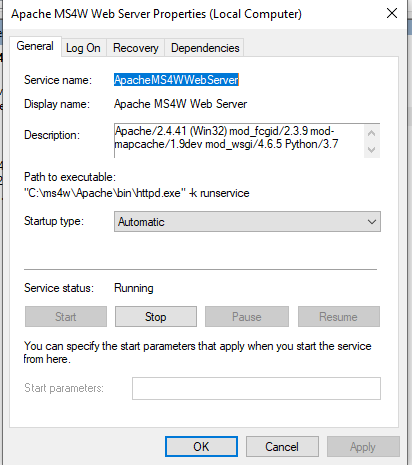
\includegraphics[width=4cm]{figures/1174017/4/7.png}
		\centering
		\caption{Pengaturan Service Apache MS4W Web Server}
    \end{figure}
\end{enumerate}
\subsection{Pengujian}
\begin{enumerate}
  \item Masuk Ke folder httpd.d yang ada di folder ms4w
  \hfill\break
    \begin{figure}[H]
		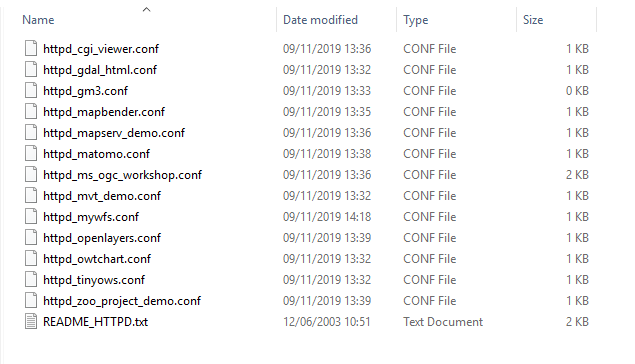
\includegraphics[width=4cm]{figures/1174017/4/Pengujian1.png}
		\centering
		\caption{Isi Folder httpd.d}
    \end{figure}
  \item Buat sebuah file dengan nama httpd mywfs conf
  \hfill\break
    \begin{figure}[H]
		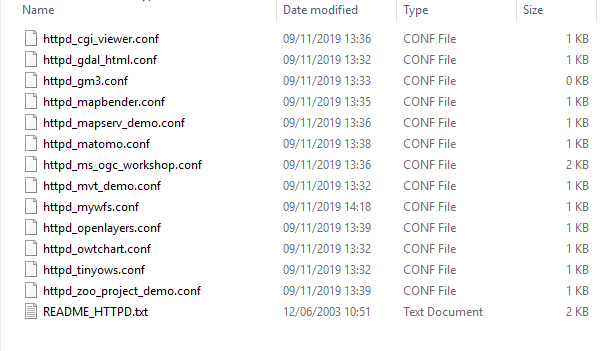
\includegraphics[width=4cm]{figures/1174017/4/Pengujian2.png}
		\centering
		\caption{Membuat file baru}
    \end{figure}
  \item Buka file httpd mywfs conf yang baru dibuat dan ubah isinya menjadi seperti berikut
  \hfill\break
    \begin{figure}[H]
		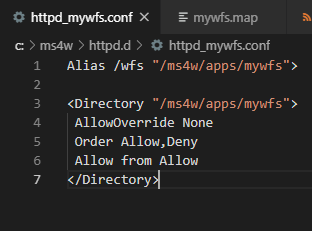
\includegraphics[width=4cm]{figures/1174017/4/Pengujian3.png}
		\centering
		\caption{Konfigurasi File Tersebut}
    \end{figure}
  \item Buka Folder apps yang ada di folder ms4w
  \hfill\break
    \begin{figure}[H]
		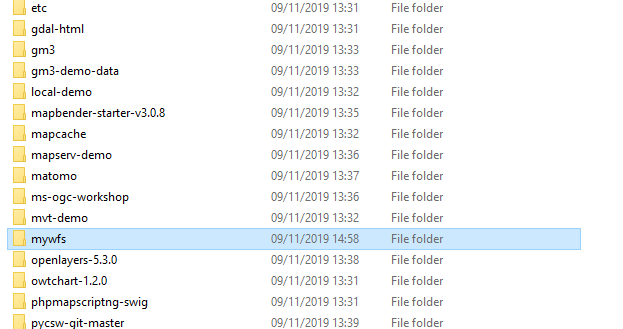
\includegraphics[width=4cm]{figures/1174017/4/Pengujian4.png}
		\centering
		\caption{Isi Folder Apps}
    \end{figure}
  \item Buat sebuah folder baru disana dengan nama mywfs,karena sebelumnya menyeting di httpd mywfs conf nya seperti itu
  \hfill\break
    \begin{figure}[H]
		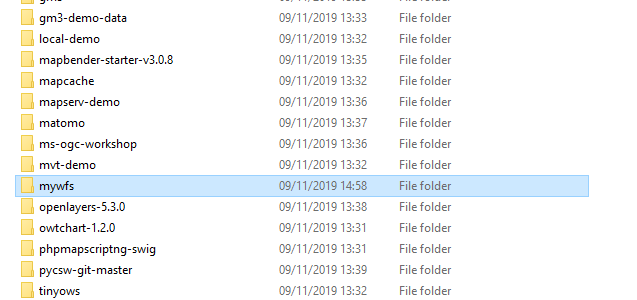
\includegraphics[width=4cm]{figures/1174017/4/Pengujian5.png}
		\centering
		\caption{Membuat folder baru}
    \end{figure}
  \item Di dalam folder mywfs buat file baru dengan nama mywfs.map
  \hfill\break
    \begin{figure}[H]
		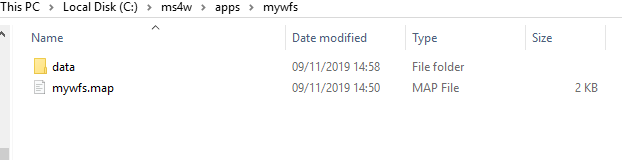
\includegraphics[width=4cm]{figures/1174017/4/Pengujian6.png}
		\centering
		\caption{Membuat file baru}
    \end{figure}
  \item Modifikasi isinya menjadi sebagai berikut
  \hfill\break
    \begin{figure}[H]
		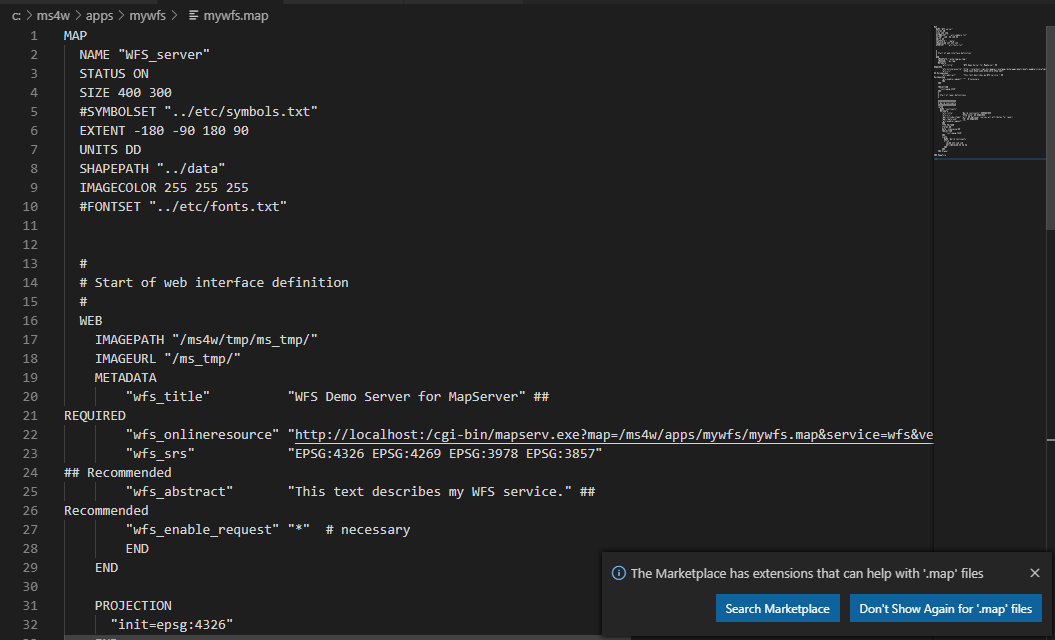
\includegraphics[width=4cm]{figures/1174017/4/Pengujian7.png}
		\centering
		\caption{Isi mywfs.map 1}
    \end{figure}
  \item Kemudian Buka Browser dan \href{http://localhost:8080/cgi-bin/mapserv.exe?map=/ms4w/apps/mywfs/mywfs.map&SERVICE=WFS&VERSION=1.0.0&REQUEST=GetCapabilities}{Klik Ini}, Karena kalo diketik manual kepanjangan
  \item Nanti akan muncul tampilan XML
  \hfill\break
    \begin{figure}[H]
		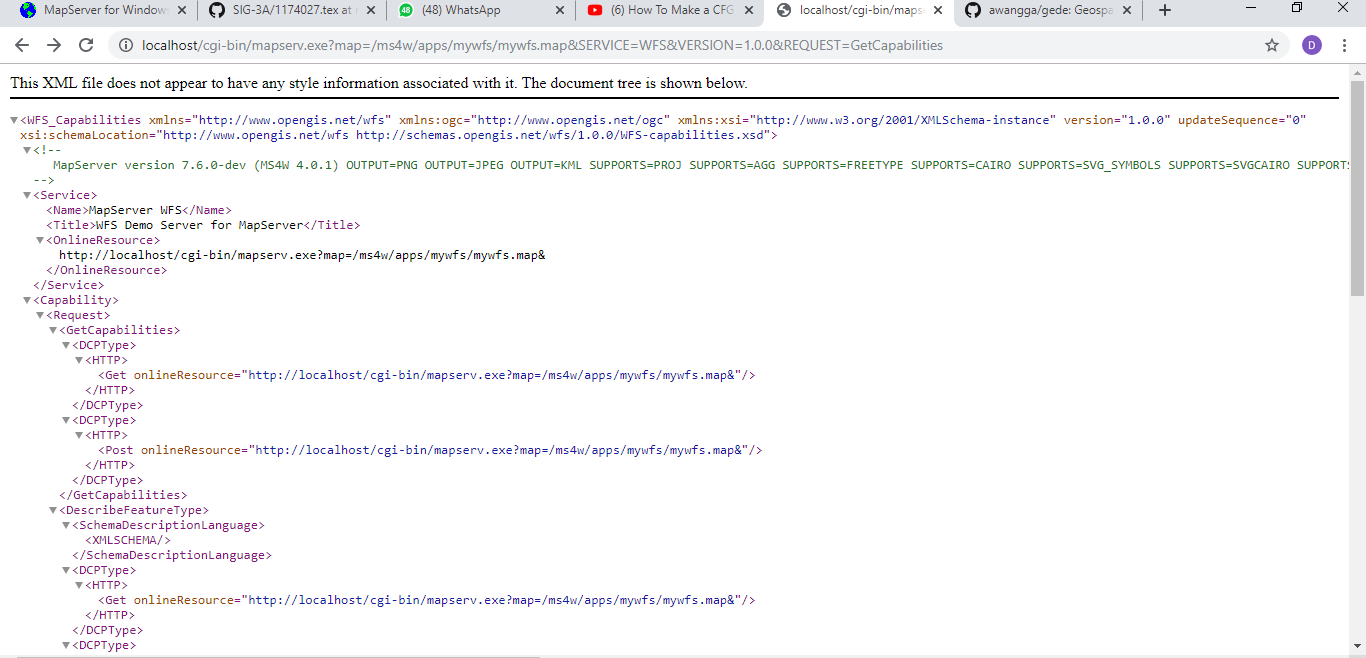
\includegraphics[width=4cm]{figures/1174017/4/Pengujian8.png}
		\centering
		\caption{Tampilan Web}
    \end{figure}
  \item Kemudian Copy dan Buat file baru dengan nama sesuaikan dengan .shp nya dan extensinya .xml
  \item Simpan didalam folder bersama dengan shp filenya
  \hfill\break
  \begin{figure}[H]
  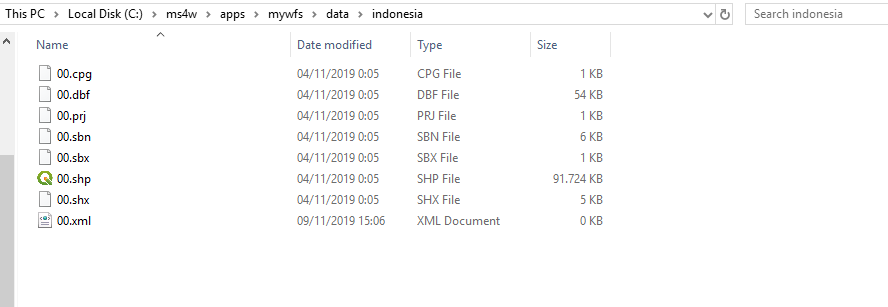
\includegraphics[width=4cm]{figures/1174017/4/xml.png}
  \centering
  \caption{File shp dengan XML}
  \end{figure}
  \item Dan sekarang buka file .shp nya, dan lihat hasil nya
  \hfill\break
  \begin{figure}[H]
  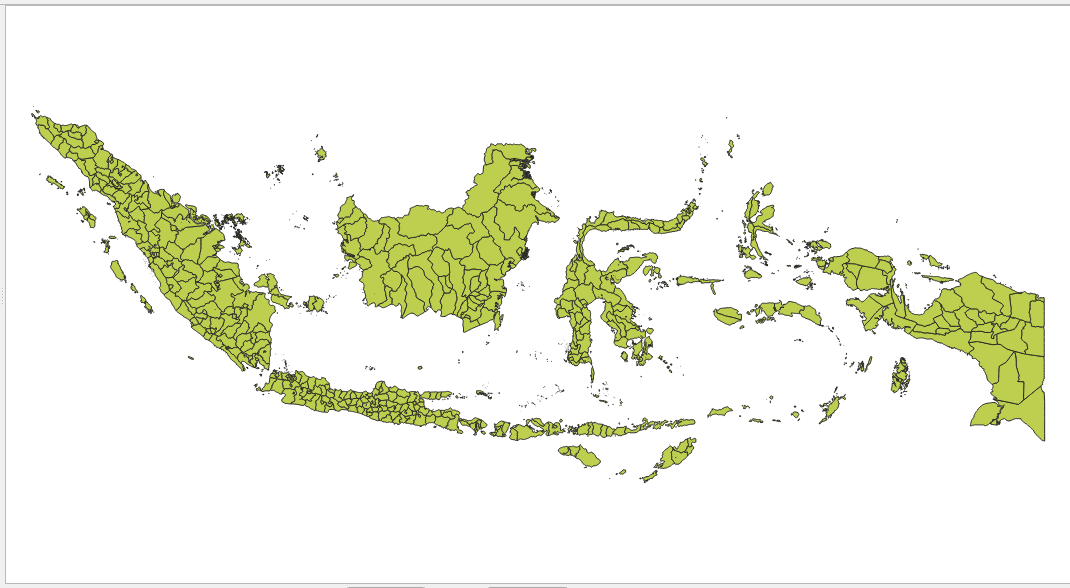
\includegraphics[width=4cm]{figures/1174017/4/map.png}
  \centering
  \caption{Hasil}
  \end{figure}
\end{enumerate}
\subsection{Link Youtube}
\href{https://youtu.be/ZSQA2gUXsuc}{Klik disini}